\documentclass[output=paper,hidelinks]{langscibook}
\ChapterDOI{10.5281/zenodo.13347674}

\author{Gerhard Jäger\affiliation{University of Tübingen}}

\title{Can language evolution lead to change for the worse?}

\abstract{Can languages change for the worse? What does it actually mean for a language to   be worse than another one? This chapter approaches this question from the point of view   of evolutionary theory. It is argued that evolving systems can be compared with regard  to their \emph{fitness}, and ``better'' can be translated as ``more fit''. Seen this  way, the initial question is an instance of the overarching problem \emph{Can evolution    reduce fitness?}  While the general answer to this question is \emph{yes}, it is  argued that this is of little interest with regard to languages as a whole, since their  fitness is mostly determined by extra-linguistic factors. However, it is shown that  there are at least three scenarios where individual linguistic items can be replaced by  less fit competitors during language change: (1) Inflationary use of extravagant  expressions, (2) systematic directed replication errors, and (3) evolutionary drift in  small populations.}



\IfFileExists{../localcommands.tex}{
  \addbibresource{../localbibliography.bib}
  \usepackage{tabularx,multicol}
\usepackage{url}
\urlstyle{same}

\usepackage{listings}
\lstset{basicstyle=\ttfamily,tabsize=2,breaklines=true}

\usepackage{langsci-optional}
\usepackage{langsci-lgr}
\usepackage{langsci-gb4e}
% \usepackage{langsci-textipa}

\usepackage{csquotes}
\usepackage{multirow}
\usepackage{colortbl}
\usepackage{ulem}
\usepackage{graphicx}
\usepackage{amsmath}
\usepackage{nicefrac}
\usepackage{tabto}
\usepackage{subcaption}
\usepackage{enumitem}
\usepackage{subcaption}


\usepackage{siunitx}
\sisetup{detect-weight=true, detect-family=true, detect-all, input-symbols={\%}, free-standing-units,group-digits=false,detect-inline-weight=math}

\usepackage[linguistics, edges]{forest}
\usetikzlibrary{matrix, arrows, arrows.meta}

\usepackage{pgfplots}
\usepgfplotslibrary{colorbrewer}
\pgfplotsset{cycle list/Dark2-4}

\usepackage{derivative}
\usepackage{langsci-branding}

  
\AtBeginDocument{%
  \SetupAffiliations{output in groups = false, 
                     separator between two = {\bigskip\\},
                     separator between multiple = {\bigskip\\},
                     separator between final two = {\bigskip\\}
                   }%
}

\newfontfamily\cjkfont
  [Scale=MatchLowercase]{SourceHanSerifSC-Regular.otf}
\AdditionalFontImprint{Source Han Serif}

\newcommand{\SC}{S\=uzh\=ou Chinese}
\newcommand{\MC}{Standard Chinese}
\newcommand{\THW}{T\`{a}ih\'{u} W\'{u}}
\newcommand{\SH}{Sh\`{a}ngh\v{a}i}
\newcommand{\iz}{ɨ̻}
\newcommand{\yz}{ʉ̻}
\newcommand{\zz}{ɿ}
\newcommand{\zw}{ʮ}
\newcommand{\pri}{*\textit{i}}
\newcommand{\pry}{*\textit{y}}
\newcommand{\prien}{*\textit{jen}}
\newcommand{\pryen}{*\textit{ɥɤn}}

\newcommand{\spr}[1]{\textsuperscript{#1}}

\renewcommand{\NG}{ŋ}
\newcommand{\textsubarch}{̯}
\renewcommand{\textschwa}{ə}
\renewcommand{\textprimstress}{ˈ}
\renewcommand{\textltailn}{ɲ}

\renewcommand{\textbabygamma}{\textramshorns}
\newcommand{\textramshorns}{ɤ}
\renewcommand{\textbardotlessj}{ɟ}
\renewcommand{\textbari}{ɨ}
\renewcommand{\textbeta}{β}
\renewcommand{\textctc}{ɕ}
\renewcommand{\textdyoghlig}{ʤ}
\newcommand{\textepsilon}{ɛ}
\renewcommand{\textesh}{ʃ}
\renewcommand{\textfishhookr}{ɾ}
\renewcommand{\textglotstop}{ʔ}
\renewcommand{\textlengthmark}{}
\renewcommand{\textopeno}{ɔ}
\newcommand{\textphi}{ɸ}
\renewcommand{\textrevepsilon}{ɜ}
\renewcommand{\textrtailr}{ɽ}
\renewcommand{\textrtailt}{ʈ}
\renewcommand{\textscriptg}{ɡ}
\renewcommand{\textthorn}{þ}
\renewcommand{\textturna}{ɐ}
\renewcommand{\textturnm}{ɯ}
\renewcommand{\textturnv}{ʌ}
\renewcommand{\textyogh}{ʒ}
\renewcommand{\textramshorns}{ɤ}
\renewcommand{\textbabygamma}{\textramshorns} %babygamma obsolete
\renewcommand{\textturnm}{ɯ}

\newcommand{\tone}[1]{\textsuperscript{#1}}
\newcommand{\underarch}{\textsubarch}

\newcommand{\sg}{\textsc{sg}}


\makeatletter
\let\thetitle\@title
\let\theauthor\@author
\makeatother


\newcommand{\togglepaper}[1][0]{
%   \bibliography{../localbibliography}
  \papernote{\scriptsize\normalfont
    \theauthor.
    \titleTemp ~
    To appear in:
    Dankmar W. Enke,   Larry M. Hyman,   Johanna Nichols,   Guido Seiler \&  Thilo Weber
    Language change for the worse.
    Berlin: Language Science Press. [preliminary page numbering]
  }
  \pagenumbering{roman}
  \setcounter{chapter}{#1}
  \addtocounter{chapter}{-1}
}


\newcommand{\ilit}[1]{#1\il{#1}}
  %% hyphenation points for line breaks
%% Normally, automatic hyphenation in LaTeX is very good
%% If a word is mis-hyphenated, add it to this file
%%
%% add information to TeX file before \begin{document} with:
%% %% hyphenation points for line breaks
%% Normally, automatic hyphenation in LaTeX is very good
%% If a word is mis-hyphenated, add it to this file
%%
%% add information to TeX file before \begin{document} with:
%% %% hyphenation points for line breaks
%% Normally, automatic hyphenation in LaTeX is very good
%% If a word is mis-hyphenated, add it to this file
%%
%% add information to TeX file before \begin{document} with:
%% \include{localhyphenation}
\hyphenation{
affri-ca-te
affri-ca-tes 
Scha-den
Zú-ñi-ga
Kaj-kwa-khrat-txi
}

\hyphenation{
affri-ca-te
affri-ca-tes 
Scha-den
Zú-ñi-ga
Kaj-kwa-khrat-txi
}

\hyphenation{
affri-ca-te
affri-ca-tes 
Scha-den
Zú-ñi-ga
Kaj-kwa-khrat-txi
}

  \togglepaper[10]%%chapternumber
}{}



\begin{document}
\maketitle

\section{Introduction}

Before I can address the questions whether languages ever do change to the worse and if
so, how this can be modeled, some clarification is needed in what sense a language A can
be ``worse'' than another language B. Some ideas that spring to mind immediately are:
\begin{itemize}
\item \emph{A is less regular than B}, e.g., has many declension classes where B has just
  one, or A has many suppletive forms in its paradigms.
\item \emph{A is more complex than B}, e.g., A allows a variety of syllable structures
  while B only uses CV-structure.
\item \emph{A is harder to acquire than B}, e.g., because A's lexicon contains many
  synonyms and B's lexicon does not.
\item \emph{A is harder to use than B}. This may apply to the speaker -- perhaps because
  the words in A are generally longer than those in B -- or to the hearer, e.g., if A's
  syntactic structures lead to many local ambiguities.
\item \emph{Certain concepts or distinctions can easily be expressed in A but not in B},
  e.g., aspectual distinctions or evidentiality.
\end{itemize}

These informal notions of \emph{worse} are not necessarily mutually distinct, and the list
is far from complete. To tackle the overarching question, a more precise notion of what it
means for a language to be worse than another is needed.

An analogy from evolutionary biology might be helpful here. According to an often-quoted
phrase due to Herbert \citet[453]{spencer1875}, Darwinian evolution is based on
the ``survival of the fittest''. In Spencer's original formulation, \emph{fittest} is used
in an informal sense. A few lines later, Spencer writes: ``While one saves its life by
higher speed, another does the like by clearer vision, another by keener scent, another by
quicker hearing, another by greater strength, another by unusual power of enduring cold or
hunger, another by special sagacity, another by special timidity, another by special
courage; and others by other bodily and mental attributes'' \citep[454]{spencer1875}. So
the comparison that organism A is less fit than organism B appears to be as vague and
multi-faceted as the notion that language A is worse than language B. However, in modern
evolutionary theory the term \emph{fitness} has a precise quantitative meaning as the
\emph{expected number of offspring}. It does not apply to individual organisms but to
populations thereof, which may be defined by heritable genotypic or phenotypic
traits. \emph{Evolution by natural selection} essentially means that the average fitness
of a population of organisms increases over time.

Conceived in this way, the question \emph{Is there evolutionary change that decreases
  fitness?} has a precise meaning, and the answer is not obvious.

Extrapolating these considerations to linguistics, one might tentatively say that language
A is worse than language B if B is fitter than A. This only makes sense, though, if the
biological notion of \emph{expected number of offspring} is applicable to languages, or,
in any event, to linguistic entities. Darwin certainly held the opinion that this is the
case. In \emph{The Descent of Man}, he notes:

  \begin{quote}\sloppy
  The formation of different languages and of distinct species, and the proofs that both
  have been developed through a gradual process, are curiously parallel. [\ldots{}] Max
  Müller has well remarked: ``A struggle for life is constantly going on amongst the
  words and grammatical forms in each language. The better, the shorter, the easier forms
  are constantly gaining the upper hand, and they owe their success to their inherent
  virtue.'' To these important causes of the survival of certain words, mere novelty and
  fashion may be added; for there is in the mind of man a strong love for slight changes
  in all things. The survival or preservation of certain favored words in the struggle
  for existence is natural selection.  \hfill\hbox{\citep[465--466]{Darwin1871}}
\end{quote}
The idea that language change shares certain characteristics with biological evolution has
regained popularity in the past two decades (see for instance \citealt{croft00} and much
subsequent work) and will be taken for granted in this article. To apply the notion of
fitness to language change, however, it needs to be clarified what linguistic
\emph{offspring}, or, more generally, linguistic \emph{replication}, amounts to.

Many researchers in the field of language evolution (Croft being a prominent example) draw
inspiration from Richard Dawkins's work (e.g., \citealt{dawkins76}). According to Dawkins,
the notion of a \emph{replicator} is central for evolution, biological or otherwise. They
are ``[t]he fundamental units of natural selection, the basic things that survive or fail
to survive, that form lineages of identical copies with occasional random mutations''
\citep[253]{dawkins76}. This suggests that replicators are discrete entities replicating
(almost) faithfully. There is a multitude of prima facie candidates for the status of
``linguistic replicator'', such as I-languages (or I-grammars) in the Chomskyan sense,
E-languages, grammatical rules, constructions, words, morphemes, phonemes, etc. For all
these linguistic units, it can be argued that they are culturally replicated in some
sense, be it via language acquisition or via imitation in language use. However, unlike
the prototypical Dawkinsian replicators -- genes -- neither of them is a discrete
physical entity directly endowed with a replication mechanism.

However, the logic of Darwinian evolution via natural selection does not require the
existence of discrete replicators and (almost-)faithful replication. This is made clear
quite lucidly in the article \emph{The nature of selection} \citep{price95} by the (among
many other things) biomathematician George Price. This little-known article, written
around 1971 but only published post-humously in 1995, spells out the conceptual
underpinning of the \emph{Price equation} \citep{price70}, a mathematical model of
Darwinian evolution.

\section{The Price equation}

Price sees selection as a very general mechanism that has been studied intensely in
biology but is also at work in other domains. He writes programmatically:

\begin{quotation}
  Selection has been studied mainly in genetics, but of course there is much more to
  selection than just genetical selection.  In psychology, for example, trial-and-error
  learning is simply learning by selection.  In chemistry, selection operates in a
  recrystallisation under equilibrium conditions, with impure and irregular crystals
  dissolving and pure, well-formed crystals growing. In palaeontology and archaeology,
  selection especially favours stones, pottery, and teeth, and greatly increases the
  frequency of mandibles among the bones of the hominid skeleton.  \emph{In linguistics,
    selection unceasingly shapes and reshapes phonetics, grammar, and vocabulary.} In
  history we see political selection in the rise of Macedonia, Rome, and Muscovy.
  Similarly, economic selection in private enterprise systems causes the rise and fall of
  firms and products. And science itself is shaped in part by selection, with experimental
  tests and other criteria selecting among rival hypotheses. \hfill\hbox{(\citealt{price95}: 389;
  emphasis mine)}
\end{quotation}

In this section I will briefly recapitulate the fundamental ideas of this article and
spell out why Price's approach is useful for the study of language change. For a fuller
account, the interested reader is referred to \citet{jaeger08Price}.\footnote{See also
  \citet{frank95} for a very good overview of Price's work in evolutionary theory.}

Price distinguishes two concepts of selection: \emph{subset selection} and \emph{Darwinian
  selection}. For instance, if ten out of one hundred applicants are admitted to college,
the selected students form a subset of the total pool of applicants. Darwinian selection,
in contradistinction, is about parents and offspring, which are disjoint sets. Both
notions of \emph{selection}, however, involve two sets which are ordered in
time. Furthermore, there is a function (in the mathematical sense) mapping the later to
the former population. For subset selection, this is just the identity function. For
biological selection, this is the \emph{parent-of} function if reproduction is
asexual. For sexual selection, one has to resort to the level of genes, and the relevant
function is \emph{is a copy of}. Price's mathematical model of selection is applicable to
any scenario of this sort, i.e., two sets where one is considered to be later in time than
the former, and a function from the later into the former set. For ease of reference, I
will call the ``earlier'' set \emph{parents} and the ``later'' set \emph{offspring}.

Selection can be iterated, i.e., the offspring can become parents of another round of
selection, etc.

For the mathematical study of selection, (at least) two functions are
required: $w$ measures the amount of entities of the two sets. Formally, it maps subsets
of the parent and offspring sets to non-negative real numbers. The simplest example $w$
would be counting, mapping each finite set to its cardinality. However, $w$ can also be a
more complex measure function such as social influence, economical value etc.

The function $x$ measures some quantitative character whose evolution is being studied. It
could be the body size of organisms, the consonant-vowel ratio of a text or what have
you. Formally, $x$ maps subsets of the parent and offspring sets to real numbers.

A schematic example of such a scenario is shown in the left panel of Figure \ref{fig:1}.
\begin{figure}
  \centering
  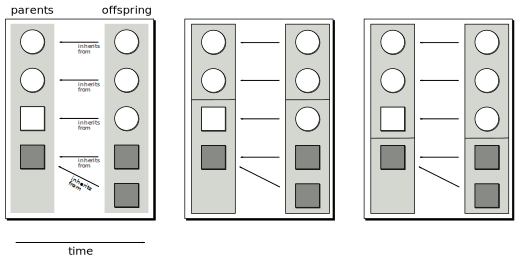
\includegraphics[width=\linewidth]{figures/figure1}
  \caption{Schematic example of selection}
  \label{fig:1}
\end{figure}

We have two populations of objects of different color and shape. The left population are
the parents and the right one the offspring. The arrows map each offspring to its parent.

In the next step, the parent population is partitioned according to some criterion. The
middle panel of Figure \ref{fig:1} partitions it according to shape and the right panel
according to color. The parent-of function induces a corresponding partition in the
offspring population. Note that the third offspring in the middle panel is placed in the
group corresponding to square-shaped parents, even though it is round rather than
square-shaped, because its parent is square-shaped.

The \emph{fitness} of a group, in the technical sense, is the amount of offspring in that
group as measured by $w$, divided by the amount of parents in the corresponding
group. Formally, if $w_i$ denotes the amount of group $i$ among the parents and $w'_i$ the
amount of the corresponding group among the offspring, the fitness $f_i$ of group $i$ is
defined as $f_i = w'_i/w_i$.

If we assume that $w$ simply counts the objects in our example, the fitness of the round
parent objects and their offspring is $\nicefrac{2}{2} = 1.0$, and $\nicefrac{3}{2} = 1.5$
for the square-shaped parents plus offspring. So the square-shaped parent objects have a
higher fitness than the round ones, because they have, on average, more offspring.

For the grouping according to color, as shown in the right panel, we have a fitness of
$\nicefrac{3}{3}=1.0$ for the white and $\nicefrac{2}{1}=2.0$ for the gray objects.

The total fitness of the population, $f$, is defined as the amount of offspring divided
by the amount of parents. In our example this is $\nicefrac{5}{4}=1.25$, regardless of the
grouping structure.

Regarding the function $x$, for a group $i$, $x_i$ is defined as the value of the parent
group $i$ under $x$, divided by $w_i$. In other words, $x_i$ is the density of $x$ in
group $i$. Analogously, $x'_i$ is the density of $x$ in the corresponding offspring group
$i$. For the whole population, $x$ and $x'$ represent the average density of $x$ among
parents and offspring respectively. The notions $\Delta x_i = x'_i - x_i$ and $\Delta x =
x'-x$ refer to the groupwise and global difference in the density of $x$ between offspring
and parents.

In our example, let us suppose that the function $x$ counts the number of gray objects in
a set. Then we have $x=\nicefrac{1}{4}=0.25$ and $x'=\nicefrac{2}{5}=0.4$, so
$\Delta x = 0.15$.

Under the groupings both in the middle and the left panel, $x_1 = x'_1 = \Delta x_1 = 0$,
since there are no gray objects on either of the upper groups. For the lower groups, we
have $x_2=\nicefrac{1}{2}=0.5$, $x'_2=\nicefrac{2}{3}=0.\overline{6}$ and
$\Delta x_2 = 0.1\overline{6}$ in the middle panel, and $x_2 = x'_2=1$, $\Delta x_1=0$ in
the right panel.

The quantity $w_i/w$ can be interpreted as the \emph{probability} of group
$i$. With this move, it follows from the definitions that%
\footnote{Here is the derivation: By definition, $\Delta x = x'-x$, and
  $x' = \sum_i w'_i x'_i/\sum_i w'_i$. As $w'_i = f_i w_i$,
  $x' = \sum_i w_i f_i x'_i/fw = \mathrm{E}(fx')/f$. Hence
  $f\Delta x = \textrm{E}(fx') - fx$. This is the left-hand side of the equation.

  By definition and elementary equivalences,
  $\mathrm{Cov}(f, x) = \mathrm{E}(fx) - \mathrm{E}(f)\mathrm{E}(x) = \mathrm{E}(fx) -
  fx$, and $\mathrm{E}(f\Delta x) = \mathrm{E}(fx' - fx) = \mathrm{E}(fx') - E(fx)$. So
  the right-hand side of the equation sums up to $\mathrm{E}(fx') - fx$ as well.%
}
\begin{equation}
f\Delta \mathrm{E}(x) = \mathrm{Cov}(f, x) + \mathrm{E}(f\Delta x).\label{eq:1}
\end{equation}


This is the celebrated \emph{Price equation} (first published in \citealt{price70}). Here,
$\mathrm{Cov}$ and $\mathrm{E}$ denote the \emph{covariance} and the \emph{expected value}
in the sense of probability theory.

The equation is a tautology; it results directly from some algebraic manipulation of the
assumptions. Its importance lies in the conceptual clarity it provides. The left-hand side
holds the total change in the average value of $x$ between parent and offspring
generation, multiplied by overall fitness. This overall change is split into two
components on the right-hand side. The first term, $\mathrm{Cov}(f, x)$, covers the
contribution of between-group \emph{selection} to the change in $x$. If $x$ strongly
covaries with fitness $f$, selection will favor an increase of $x$ over time. Conversely,
if high values of $x$ are associated with low fitness and vice versa, selection leads the
average value of $x$ to shrink.

This is not the full story though. The second term, $\mathrm{E}(f\Delta x)$, captures the
change of $x$ between parents and offspring \emph{within groups}. If the average value of
$x$ within a group $i$ is unchanged between parents and offspring, $\Delta x_i = 0$. If
this holds for all groups, $x$ is replicated faithfully. Provided that the external
circumstances do not change, the second term becomes 0. However, if replication is not
fully faithful or the environment changes, the term may be non-negligible. So one way to
interpret the Price equation is to say that it separates evolutionary change into the
effect of natural selection and the effect of unfaithful replication and a changing
environment.

It is important to point out though that this distinction between selection and
within-group change depends on the assumed grouping of the parent population. Since this
is imposed by the modeler rather than being empirically determined, this distinction is an
analytical tool, not something which is objectively given.

To bring this point home, consider again the example in Figure \ref{fig:1}. Average
fitness $f$ is $1.25$ and the change in the average proportion of gray objects is
$\Delta x = 0.15$. So regardless of the grouping, the left-hand side of the Price equation
is:
\[f\Delta x = 1.25 \cdot 0.15 = 0.1875\]

For the right-hand side of the equation, the grouping structure makes a difference.  In
the middle panel, the populations are grouped according to the parents' shape. The
character of interest $x$, changes from $0.5$ to $0.\overline{6}$ between parents and
offspring for the square-shaped group, so it is not faithfully replicated. Therefore the
second term is non-negligible. Numerically, we have
\begin{eqnarray*}
  \mathrm{Cov}(f, x) &=& 0.0625\\
  \mathrm{E}(f x) &=& 0.125
\end{eqnarray*}

In the left panel, objects are grouped according to parents' color. Here the proportion of
gray objects remains constant between parents and offspring for both groups, so the second
term becomes $0$. Carrying out the calculation gives
\begin{eqnarray*}
  \mathrm{Cov}(f, x) &=& 0.1875\\
  \mathrm{E}(f x) &=& 0
\end{eqnarray*}\largerpage[-1]

So according to the first grouping, we find moderate between-group selection for grayness
(of magnitude $0.0625$) and unfaithful within-group replication favoring
grayness. According to the second grouping, there is faithful replication and stronger
between-group selection for grayness (of magnitude $0.1875$). Both conceptualizations
describe the same dynamics, though. In both cases, the sum of the two terms equals the
left-hand side of the equation.

The explicit focus of the Price equation on the grouping structure makes it well-suited to
study hierarchical selection, e.g., the relative strength of between-individual and
between-groups selection. Also, it can be used to capture the effects of directed
mutations via the second term.

A major advantage of Price's approach is its generality. It leaves the modeler complete
freedom to decide what kind of dependency between stages of a system is considered as
parent-of relation, and how populations are structured into groups. The question what
\emph{is} a replicator in linguistics is meaningless in this context. It is up to the
modeler to decide what is \emph{considered as} unit of selection.

To return to the mathematical detail, in the limiting case where selection is iterated
many times and the time interval between successive generations is so short that time can
be approximated as continuous, the Price equation becomes the differential equation (see
\citealt{price72b} for the derivation)
\begin{equation}
\odv{\mathrm{E}(x)}{t} = \mathrm{Cov}(f, x) + \mathrm{E} \left(\odv{x}{t}\right).\label{eq:2}
\end{equation}



\section{Fisher's fundamental theorem and evolutionary change to the worse}

In his landmark book \emph{The Genetical Theory of Natural Selection} (originally
published in 1930), Ronald Aylmer Fisher -- one of the founders both of population
genetics and of statistics -- postulated what he called the \emph{fundamental theorem of
  natural selection:}
\begin{quote}
  The rate of increase in fitness of any organism at any time is equal to its genetic
  variance in fitness at that time.\hfill\hbox{\citep[35]{fisher1999}}
\end{quote}

If higher fitness is read as ``better'' and vice versa, this seems to suggest that there
cannot be biological evolution to the worse. A moment's thought reveals, however, that
this ``theorem'' cannot be quite right in its literal interpretation. If \emph{variance in
  fitness} is taken in its obvious mathematical interpretation, this quantity cannot be
negative. In fact, it has to be positive in any population that is not fully homogeneous
with respect to fitness.\footnote{By the term \emph{organism}, Fisher must refer to
  populations of organisms, since an individual organism cannot have variance in fitness.}
So according to the theorem, the \emph{rate of increase in fitness} must be non-negative,
and in fact positive in almost all cases. Once a population has a fitness $> 1$, fitness
must remain $> 1$, and this entails that such a population will keep growing
indefinitely. This is of course inconsistent with the observation that populations never
grow forever.

In \citet{price72a} it is spelled out how Fisher's theorem is to be understood, and a
simple proof is given. It can easily be shown to be corollary of the Price equation.

Consider the continuous-time version of the Price equation given in Equation
(\ref{eq:2}). The quantity $x$ can be any quantitative character, including fitness. If
one replaces $x$ with $f$, one gets
\begin{equation*}
  \odv{\mathrm{E}(f)}{t}     = \mathrm{Cov}(f, f) + \mathrm{E}\left(\odv{f}{t}\right)
                             = \mathrm{Var}(f) + \mathrm{E}\left(\odv{f}{t}\right)
\end{equation*}

Recall that the first term on the right-hand side captures the change due to selection. So
what this formulation says is that the part of change in fitness \emph{that is due to
  selection} equals the variance in fitness. This variance is virtually always positive,
but this may be offset by the second term, which tracks the within-group change in fitness
from parents to offspring. This term may be negative for two reasons. First, replication
may be unfaithful, and this change -- perhaps due to a deleterious mutation -- decreases
fitness. Still, even if replication is fully faithful, the term may be negative. To see
why, recall that the change in fitness is the difference in fitness between offspring and
parents, and fitness is the expected number of offspring. Even if the offspring is an
exact copy of its parent, it fitness may be lower because \emph{the environment may have
  changed.} Similar to generals that proverbially always fight the last war, evolution
favors change from parents to offspring generation that would benefit the offspring if
they were to live in the parents' environment, but it may or may not benefit them in their
actual environment. \citet[41]{fisher1999} called this effect the ``deterioration of
the environment''.

To return to the issue whether there may be evolutionary change to the worse, the answer
is: Yes, populations may change to the worse in evolution if the deleterious effects of
unfaithful replication and of the deterioration of the environment are stronger than the
effect of natural selection.\largerpage[-1]

A well-known example of deterioration of the environment is the prisoner's dilemma. Recall
that in this kind of game, there are two types of players, \emph{cooperators} $C$ and
\emph{defectors} $D$. The utility matrix for the game is
\begin{center}
  \begin{tabular}{lll}
    \toprule
        & $C$ & $D$ \\\midrule
    $C$ & 2,2 & 0,3 \\
    $D$ & 3,0 & 1,1 \\\bottomrule
  \end{tabular}
\end{center}
where the first number in each cell is the utility of the row player and the second one of
the column player. The maximal overall utility that can be achieved is 4 if both players
are $C$, and it is lowest with 2 if both play $D$. Still, it is rational to play $D$
because $D$ always incurs a higher utility than $C$, no matter which strategy the opponent
plays.

This pessimistic prediction carries over under an evolutionary interpretation of the game
where utility is interpreted as fitness. Suppose we have a large population consisting
entirely of $C$ players. Then there is a mutation, leading to a single $D$-player. This
mutant will have a fitness of 3 while the rest of the population has fitness of $\leq
2$. Therefore $D$ will spread over the generations, and the overall population will
approach a pure $D$ state. So the average fitness of the population starts at 2 and
converges to 1. Still, if one of the $D$-players were placed in the original environment
of a pure $C$-population, its fitness would be 3. The decrease in average fitness is a
result of the changing population composition.

\section{Deterioration of the linguistic environment}

The various notions of linguistic replication mentioned above -- replication of
I-languages, E-languages, grammatical rules, constructions, words, morphemes etc.\ -- can
all be accommodated within the Pricean framework. Consider the generative notion according
to which linguistic replication primarily proceeds via first language acquisition of
syntactic parameters (cf., e.g., \citealt{lightfoot99}). In the simplified case where each
infant acquires language from exactly one teacher, each acquired parameter value can be
considered the offspring of the teacher's corresponding value. In a more realistic
scenario, a learner has more than one teacher though, and there is a probabilistic
relation from teacher's to learner's parameter values. This can be fitted into Price's
framework if we replace $x$, $f$, and $w$ by their expected values.

Similar considerations apply to usage-oriented notions of linguistic
replication. Following \citet{bybee06}, exemplars, i.e., memory traces, of linguistic
experiences can be seen as forming the populations selection operates on. As with
syntactic parameters, there is no unique map from offspring to parent, so formally, the
underlying probability space over exemplars would be the populations in the formal sense.

Taking the latter perspective, the fitness of an exemplar would then amount to the
expected number of later exemplars that it spawns. In other words, an exemplar is accessed
in the production of an utterance by the speaker, and this utterance is stored as a new
exemplar by the listener(s) and perhaps by the speaker herself. While the number of
listeners is a non-linguistic random variable that can be averaged out when considering
the expected fitness of an exemplar \emph{type}, the crucial fitness-inducing features are
(a) the frequency of situations where the speaker wants to make an utterance where the
exemplar provides a suitable precedence, (b) the ease of access from memory (as compared
to other suitable exemplars), and (c) the likelihood that the resulting utterance is
stored as an exemplar in the listener's memory. It is easy to recognize the well-known
notions of speaker economy in (b) and hearer economy in (c).

The overall fitness of a population of exemplars within a speech community, however, is no
linguistically meaningful quantity, as it depends on the number of community members and
their verbosity, not on language internal features. In this sense, a language --
conceived as the totality of linguistic exemplars stored in the minds of the language users -- becomes fitter if the total amount of usage of the language increases (and vice
versa). This can happen because the language community expands or because people increase
their linguistic activity. In this sense, language change to the worse, i.e., decrease in
linguistic fitness, occurs if and only if the usage of a language shrinks, for whatever
reason. This, however, has arguably little to do with the language's properties as such,
and is therefore not a helpful answer to the overarching question of this
volume.\footnote{One reviewer remarked that in situations of direct language competition
  in multilingual contexts, selection between languages takes place, and factors like
  learnability or expressivity might have an impact on the strength of selection between
  languages. This is a relevant aspect that will not be pursued further here.}


To formulate it in another way, if extralinguistic and sociolinguistic factors are
averaged over, languages do not change to the better or to the worse as long as they serve
the language users' communicative needs. However, we may ask whether certain slots within
the language system can change to the worse, in the sense of losing fitness.

This is exactly what is happening in the initial stages of grammaticalization, as
conceived by \citet{Haspelmath1999}. He assumes (\citeyear[1055]{Haspelmath1999}) the following schematic structure of this
process:

\begin{quote}
\begin{enumerate}[label=\alph*., leftmargin=*]
  \item A speaker says YB$_{\mathrm{L}}$Z where s/he could have said
    YA$_{\mathrm{F}}$Z [...]. (X$_{\mathrm{L}}$ = lexical element; X$_{\mathrm{F}}$=functional
    element).
  \item Other speakers follow him/her and say YB$_{\mathrm{L}}$Z, too [...].
  \item B$_{\mathrm{L}}$ increases in frequency in the community's speech, because B's
    new meaning is more basic to discourse [...].  
  \item Because of its high frequency, B becomes more predictable.
  \item Because of its predictability, B is pronounced in a reduced manner by many
    speakers [...].  
  \item Because of its high frequency, B (which is now B$_{\mathrm{F}}$) is
    increasingly automated/routinized in the speaker's mind [...]; automated processing
    entails features such as merger with adjacent elements; obligatory use in certain
    contexts; fixed position; etc.; [...].  
  \item Through habituation, the meaning contribution of B is no longer perceived as
    pragmatically salient.
\end{enumerate}
\end{quote}

This process is set in motion due to a conversational maxim stated in \citet{keller94},
which \citet{Haspelmath1999} dubs the maxim of ``extravagance'': ``Talk in such a way that
you are noticed.'' \citep[101]{keller94}

During stage b., the innovative item B achieves a high fitness because few existing
exemplars give rise to many copies thereof. However, during stages c.\ and d., B's fitness
decreases because a speaker choosing B has more exemplars to draw from, and B is not very
extravagant anymore. During this phase, B is \emph{getting worse}. Haspelmath aptly
compares this process with economic inflation, where an oversupply of money leads to its
devaluation.

Note that this effect applies whether or not B is phonetically reduced and/or semantically
bleached during this process. What has changed from phase a.\ to phase c.\ is the
surrounding population of linguistic exemplars, not the linguistic type. B's reduction in
fitness is an instance of deterioration of the environment in the sense described in the
previous section.

\section{Directed mutations}

Price's framework does not require replication to be faithful. (Recall, e.g., that in the
example in Figure \ref{fig:1}, the third row changes its shape from square to round.)
Changes due to unfaithful replication are also covered by the second term of the
right-hand side of the equation, just like deterioration of the environment. If copying
errors reduce fitness, this may also lead to a decrease in fitness.

Let me illustrate this point with a schematic example\footnote{This is an instance of the
  \emph{quasispecies} model from biomathematics; cf.\ \citep{eigenSchuster79}.}, which is
illustrated in Figure \ref{fig:2}.
\begin{figure}
  \centering
  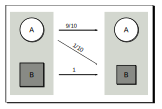
\includegraphics[width=0.6\linewidth]{figures/quasispecies}
  \caption{Schematic example of fitness loss due to directed mutations}
  \label{fig:2}
\end{figure}
Suppose we have two types of individuals, $A$ and $B$, in a population. $A$ has fitness 1
and $B$ has fitness $\nicefrac{4}{5}$. $B$ always reproduces faithfully, but there is a
$\nicefrac{1}{10}$ chance that the offspring of an $A$-individual is a mutant and has type
$B$. Suppose the population consists of $\nicefrac{2}{3}$ type $A$ and $\nicefrac{1}{3}$
type $B$. Then the variance in fitness is $\nicefrac{2}{225}$. The expected change in
fitness for type $A$ is $\nicefrac{-1}{50}$ (since there is a 1 in 10 chance that the
offspring has type $B$ and therefore fitness $\nicefrac{4}{5}$ rather than 1), while the
expected change in fitness for type $B$ is 0. So the expected change in fitness due to
unfaithful mutation is $\nicefrac{-1}{75}$. This amounts to a net change in population
fitness of $\nicefrac{-1}{225}$. (This system will eventually settle in an equilibrium
where both types are equally abundant.)

A linguistic instance of this effect is phonetic reduction. Consider, e.g., the \ili{English}
word \emph{fifteen}, pronounced /ˈfɪf.tiːn/. Analogously to \emph{fourteen, sixteen,
  seventeen} etc., the regular word for $10+5$ should be \emph{fiveteen}
(/ˈfaɪv.tiːn/). Arguably, the monophtongization of the vowel and subsequent consonant
devoicing in /ˈfɪf.tiːn/, as compared to the regular formation /ˈfaɪv.tiːn/, are the
result of phonetic reduction. It is well-known that phonetic reduction is the more likely
the more frequent a word is (see, e.g., \citealt{ernestus2000}). \citet{krifka07} observes
that round number words are ambiguous between a precise and a vague interpretation, while
non-round numerals only have the precise interpretation.\footnote{I owe the example
  regarding \emph{fifteen} to Manfred Krifka, p.c.} Therefore it stands to reason that
round number words such as \emph{fifteen} words are more frequent in conversation than
comparable non-round words like \emph{fourteen} or \emph{sixteen}. In fact, according to
the Google Ngram Viewer\footnote{\url{http://books.google.com/ngrams}, accessed on
  September 10, 2019.}, \emph{fifteen} was consistently more frequent then either
\emph{fourteen} or \emph{sixteen} in \ili{English} language books between 1800 and 2000. The
plot is given in Figure \ref{fig:3}.

\begin{figure}
  \centering
  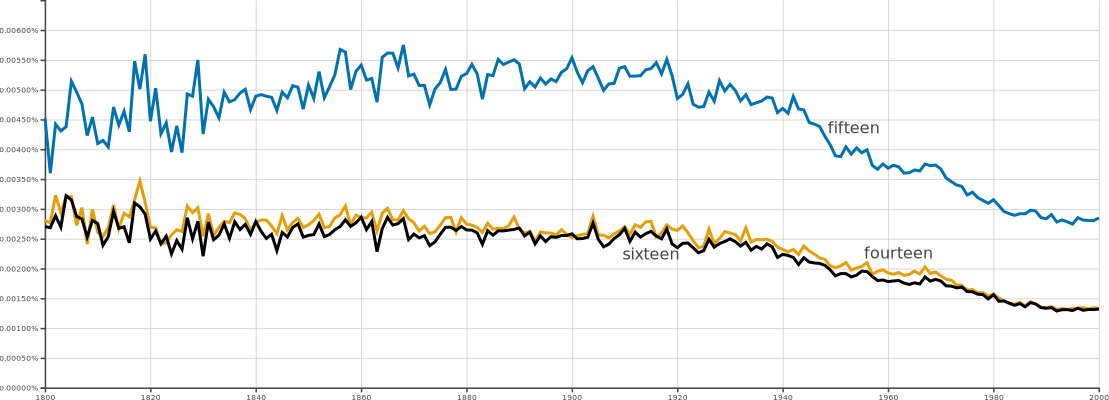
\includegraphics[width=\linewidth]{figures/ngrams}
  \caption{Google Ngram search for \emph{fourteen} (orange), \emph{fifteen} (blue) and
    \emph{sixteen} (black).}
  \label{fig:3}
\end{figure}

The regular formation \emph{fiveteen} is easier to acquire for language learners than the
irregular \emph{fifteen}, so it arguably has a higher fitness. However, hypoarticulation
of \emph{fiveteen} is apt to lead to altered replication; many exemplars of
\emph{fiveteen} spawn \emph{fifteen}-offspring. This eventually led to the the
entrenchment of the phonetically reduced form \emph{fifteen}. So here we have a case where
in a competition between a fitter and a less fit item, the latter wins out because there
is systematic altered replication to its favor.

\section{Random drift}

A third scenario where the fitness of a population can decrease despite the force of
selection is \emph{random drift}. This effect becomes negligible as population size
increases but can be substantial in small populations.

Again I will give a simple example for illustration. Suppose a population consists of two
types of individuals, types $A$ and $B$, with fitness $f_A$ and $f_B$ respectively such
that $f_A < f_B$. In this scenario, both sub-populations will grow indefinitely, even
though the relative size of the $A$-subpopulation will shrink in comparison to the
$B$-subpopulation. But now suppose $f_A$ and $f_B$ are random variables rather than being
fixed. The exact number of offspring of an $A$-individual may depend on all sorts of
random circumstances, and it is only known that its \emph{expected value} is $f_A$ (and
likewise for $B$-individuals). If the total population size is finite and limited, there
is a positive probability that a mixed population will evolve towards a pure
$B$-population, even though $A$ has a higher expected fitness.

A simple model of this principle is the \emph{Moran process} \citep{moran58}. It assumes a
finite population of fixed size $N$. At each time step, one individual is picked at random
from the population, and a copy of it is made. Then a random individual is picked (which
could be the same as the first) and eliminated, and the copy of the first individual
assumes its place. This is illustrated in Figure \ref{fig:4}.

\begin{figure}
  \centering
  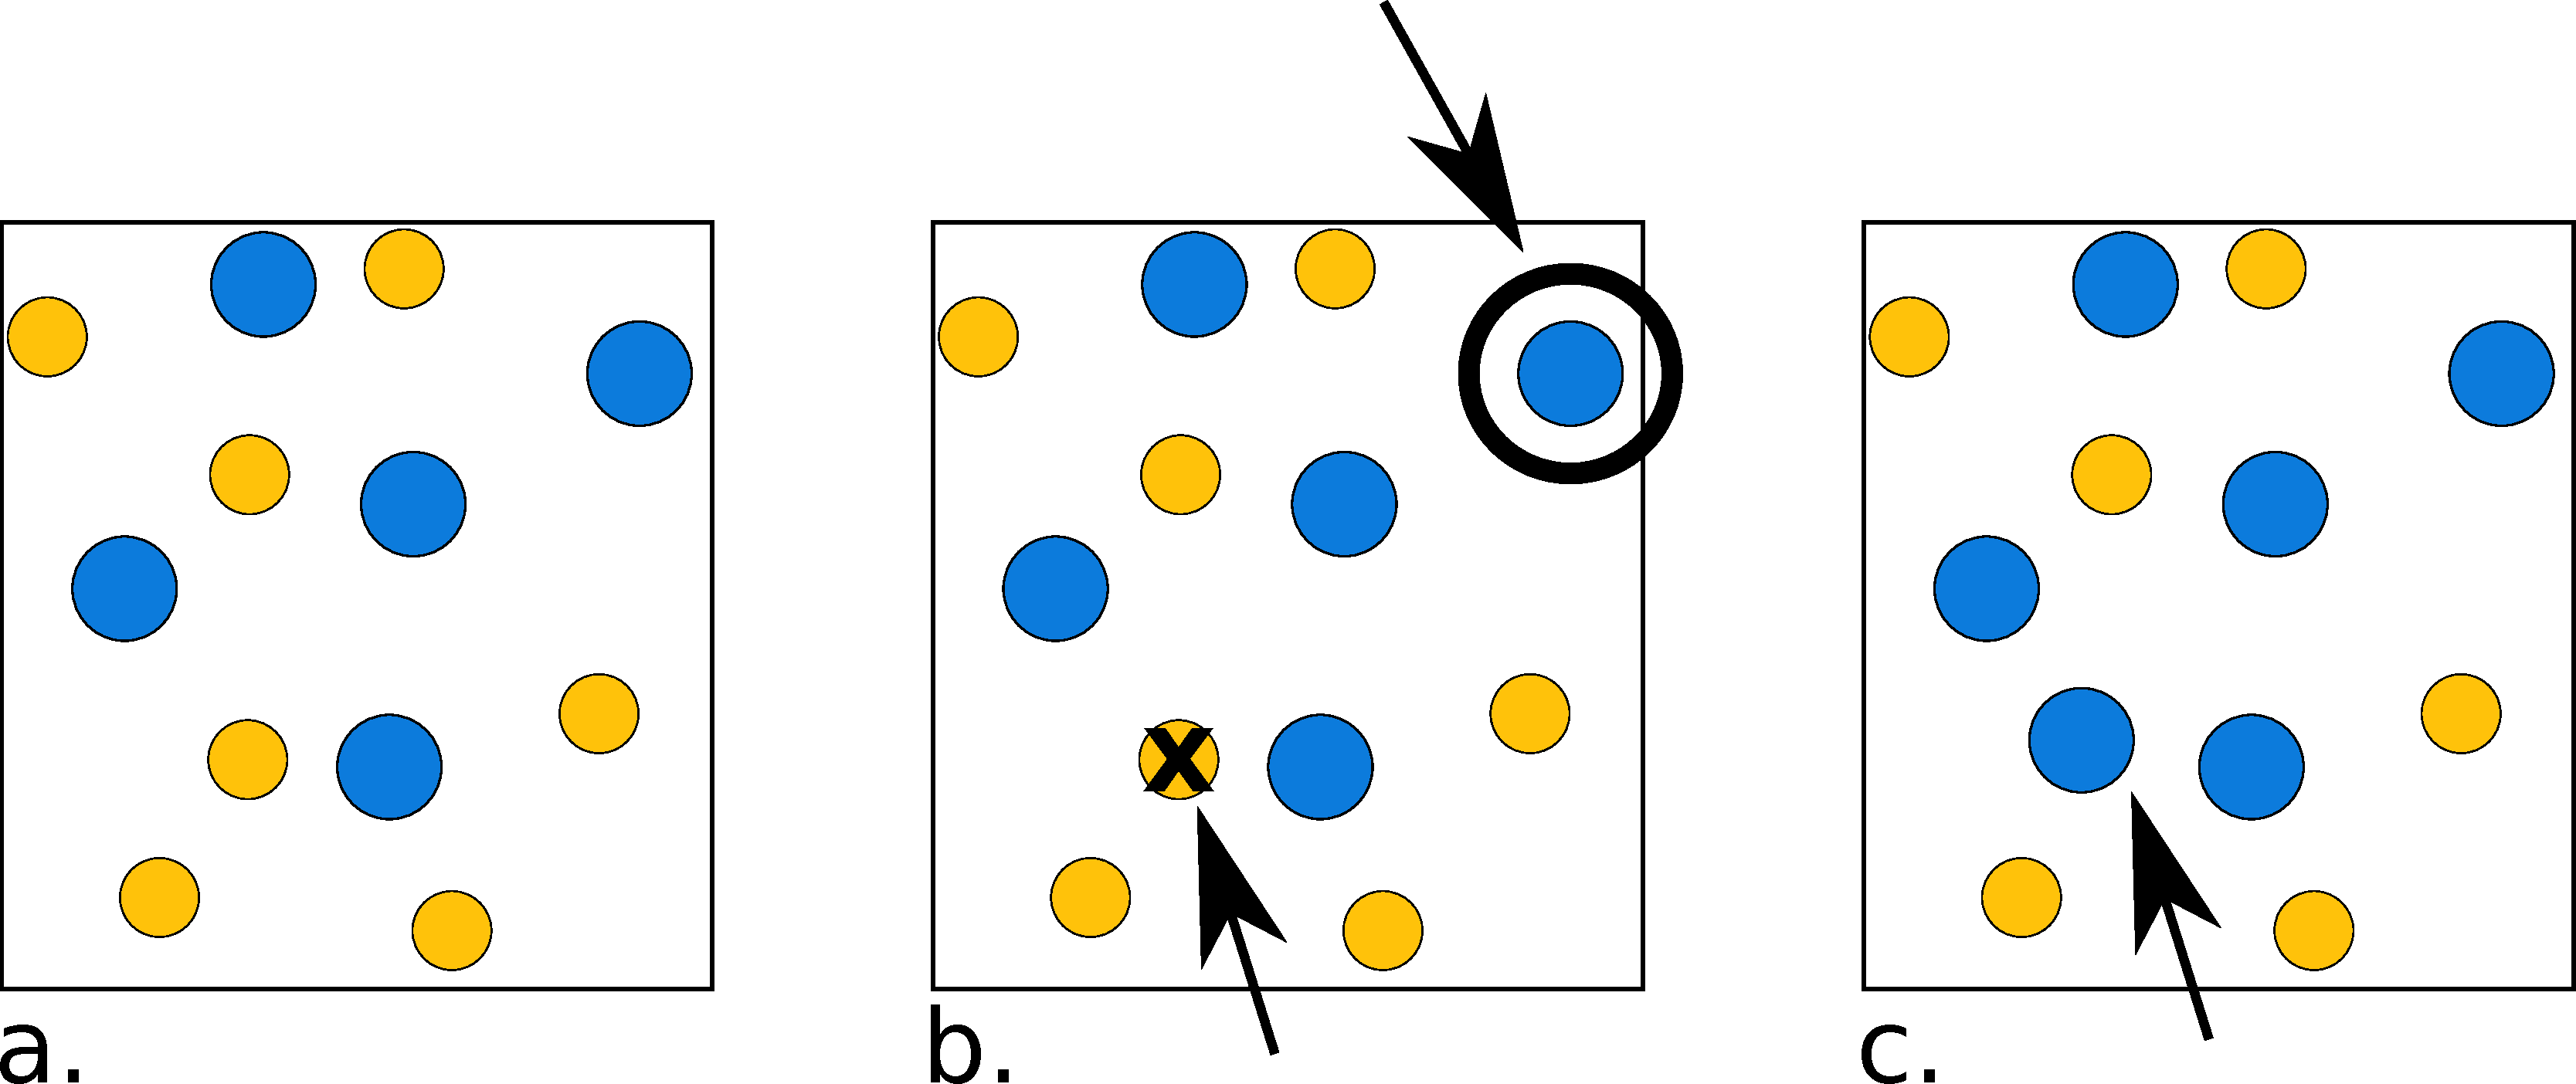
\includegraphics[width=.75\linewidth]{figures/moranProcess}
  \caption{Moran process. In a finite population (a.), an individual is chosen randomly
    for replication and one for elimination (b.). The eliminated individual is replaced by
    a copy of the replicated one (c.).}
  \label{fig:4}
\end{figure}

The probability that a given individual of type $A$ is picked for replication is $p(A)$, and
likewise for $p(B)$. Each individual is equally likely to be picked for elimination.

Now suppose a population of size $N$ consists entirely of $B$-individuals, but one
replication event introduces a mutation. This results in one $B$-individual being replaced
by an $A$-individual. No further copying errors occur. According to \citet[101]{nowak06},
the probability that the entire population is eventually replaced by $A$-individuals is
given by the formula
\begin{equation*}
  \label{eq:3}
  P(B\rightarrow A) = \frac{r^{-1} -1}{r^{-N}-1}, \mbox{where } r = \frac{p(A)}{p(B)}.
\end{equation*}

If $p(A) < p(B)$, this is the probability that the ``better'' type $B$ is replaced by the
``worse'' type $A$. As shown in Figure \ref{fig:5}, this probability can be non-negligible
if both the population and the discrepancy between $p(A)$ and $p(B)$ is small.

\begin{figure}
  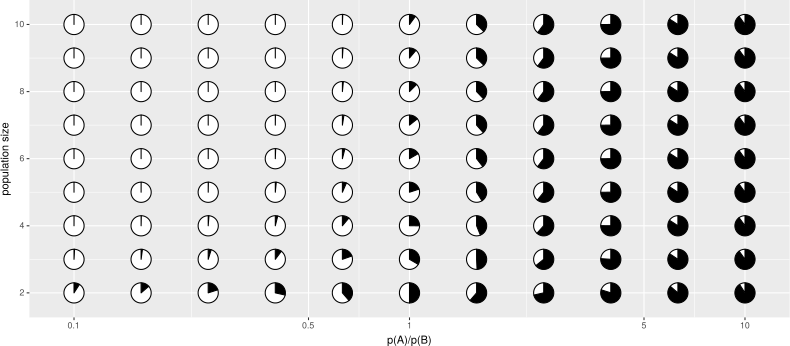
\includegraphics[width=\textwidth]{figures/weakSelection}
  \caption{Probability of a finite population of incumbents $B$ being successfully invaded
    and replaced by a mutant $A$}
  \label{fig:5}
\end{figure}

The figure also shows that even if $p(A) > p(B)$, i.e., if $A$ is better than $B$, it is
by no means certain that $A$ will replace the worse type $B$.

Instances of language change where among two competing forms, the less natural/more marked
variant occasionally wins out are not hard to come by. An example would be the general
trend in \ili{Germanic} languages to replace the strong (vowel alternation) by the weak (dental
suffix) verbal inflection. Verbs that changed from strong to weak abound, e.g.\ \ili{English}
\emph{shove} which derived from the the strong \ili{Old English}
\emph{scufan}\footnote{\url{www.etymonline.com}, accessed on April 23, 2019.} or the
\ili{German} \emph{kauen}, derived from the strong \ili{Old High German}
\emph{kiuwan}.\footnote{\url{www.dwds.de}, accessed on April 23, 2019.} However, there are
a handful of examples of the opposite trend, verbs that were originally weak but switched
to strong inflection, such as \ili{English} \emph{dive}\footnote{%
  According to \url{www.etymonline.com}, accessed on April 23, 2019:
  \begin{quotation}
    \textbf{dive (v.)}
    
    c.\ 1200, diven, ``descend or plunge headfirst into water,'' from a merger of \ili{Old English} \emph{dufan} ``to dive, duck, sink'' (intransitive, class II strong verb; past
    tense \emph{deaf}, past participle \emph{dofen}) and \emph{dyfan} ``to dip, submerge''
    (weak, transitive), from \ili{Proto-Germanic} verb \emph{*dubijan}, from PIE\il{Proto-Indo-European} \emph{*dheub-}
    ``deep, hollow'' (see deep (adj.)).

    In the merger of verbs the weak forms predominated and the strong inflections were
    obsolete by 1300. The past tense remained \emph{dived} into 19c., but in that century
    dove emerged, perhaps on analogy of \emph{drive/drove}.  [...]
  \end{quotation}} or \ili{German} \emph{schrecken}.\footnote{\url{www.dwds.de}, accessed on April 23, 2019:
  ``Das ursprünglich schwach flektierende, mit j-Suffix gebildete, intransitiv gebrauchte
  Verb ahd.\ \emph{scricken} `empor-, aufspringen, erschrecken' (um 800) [...] entwickelt
  die Bedeutung `in Schrecken geraten, erschrecken' aus [...].''} It seems plausible that
the synchronously regular weak inflection is easier to acquire by children and second
language learners and therefore has a higher fitness than the competing strong inflection
(if both exist or can be morphologically constructed). Since the population of exemplars
of a verb is finite, we expect switches from one inflectional paradigm to the other to be
possible, and the switch from strong to weak inflection to be more probable. However, the
switch from weak to strong inflection has a probability $>0$, so it to be expected to
occur occasionally.

\section{Conclusion}

This article probed the question whether languages can change to the worse from a
conceptual, modeling point of view. I argued that this question has an illuminating
analogy to the issue whether Darwinian evolution in biology can lead to the reduction of
fitness. Following much recent work in historical and evolutionary linguistics, I assume
that biological evolution and language change are two instances of an overarching
principle of evolution via replication and selection. I furthermore argued that George
Price's mathematical framework is well-suited to tackle conceptual questions like the one
discussed here. My main conclusions are:

\begin{itemize}
\item A language as a whole cannot become better or worse, in the sense of increasing or
  decreasing in fitness, as long as it is fully functional as a vehicle for communication
  in its speech community.
\item Parts of the language system can become worse in the sense that they are changed
  towards or replaced by alternatives that would be less fit than the original version
  under similar circumstances.
\item There are at least three general scenarios for how this can happen:
  \begin{enumerate}
  \item \emph{Deterioration of the environment}, e.g.\ inflationary use of originally
    extravagant forms,
  \item \emph{directed mutations}, e.g.\ in phonetic reduction, and
  \item \emph{random drift}, e.g.\ switch from weak to strong verbal inflection in
    \ili{Germanic} languages.
  \end{enumerate}
\end{itemize}

\section*{Acknowledgments}

I would like to thank the two reviewers of this chapter for helpful feedback. This
research was supported by the European Research Council (ERC) under the European Union's
Horizon 2020 research and innovation programme (Grant agreement No.\ 834050) and the
German Research Foundation (DFG-FOR 2237), which is gratefully acknowledged.

{\printbibliography[heading=subbibliography,notkeyword=this]}
\end{document}
